\section{\iflanguage{english}{Results}{Ergebnisse}}
\label{sec:results}

Using the tools available at our disposal, we have done 6 experiments. The first 6 experiments of the original paper are reproduced and above we have summarized the results and our insights from these experiments.
There are 3 main questions we wish to gain more intuition on.
First, we would like to see what would be the result of the networks losing plasticity. In an essence, what is the reason we care and what are the repurcussions of this phenomenon. In the first experiment we show that the optimizer instability under abrupt label changes will lead to a large fraction of inactive ReLU units and thus loss of representational capacity. Then we move to the second experiment and show that the Hessian spectrum and gradient covariance are affected by the optimization process and thus the geometry of the loss landscape is changed in a way that makes it harder to optimize on new objectives.

Second question we wish to answer, is to what properties would cause plasticity loss? We try to investigate the effect of long-discussed weight norm and dead-units and show that there's no direct causal relationship between these metrics and loss of plasticity. Then we move to our other experiment and try to measure the plasticity of trained networks after arbitrary learning time and see that learning speed reduces as training proceeds.

At the end we have put our efforts to verify the solutions to alleviate this issue, by trying to answer several questions. Such as would increasing the size of the network be enough, or which kind of interventions in the networks is the most beneficial. We see that unlike other regimes, in which increasing the capacity will help, in deep reinforcement learning world that we have non-stationary targets, simply increasing the size of the network has not that effect. Then we analyze the effect of few previously suggested methods, such as shrink and perturb, resetting last layer, layer-normalization and others on two architectures of simple MLPs and Vision Transformers; We have observed that the paper's claim is indeed relevant and the most effective remedies are layer normalization and categorical representations (or also known as two-hot encoding).

As a disclaimer, we would like to point out that the compute resources available to us are limited and we have to make some compromises on the size of the networks and the number of experiments we can run. We will try to reproduce the results from \citep{lyle2023understanding} as closely as possible. On some of the more compute-extensive tasks like the ones involving CNNs and Vision Transformers, we will have to reduce the number of experiments and seeds. Thus we may see an increase in variance in our results compared to the original study.


\subsection{Optimizer Instability Under Abrupt Label Changes}

The purpose of this experiment is to study how an adaptive optimizer behaves when the learning objective changes abruptly. In this setting, the network is first trained on MNIST images with randomly assigned labels. After the network has learned this mapping, the labels are randomly reassigned while the input images remain fixed.

This creates a sudden change in the underlying gradient structure of the network. The optimizer must now adapt to a new objective that is inconsistent with the previously learned one. In the case of Adam, the first- and second-moment estimates no longer accurately describe the new gradient distribution. As a result, the effective update sizes can become unstable. The experiment also shows a tuned version of Adam, which tries to mitigate this sudden change by adding a small constant.

The reproduced experiment shows that this instability can cause a large fraction of hidden ReLU units to become inactive. Once these units die, the network loses effective representational capacity and its ability to learn the new task is strongly reduced. This provides an example of plasticity loss caused by optimizer dynamics under non-stationarity.

\begin{figure}[htbp]
\centering
% Replace with reproduced Figure 1
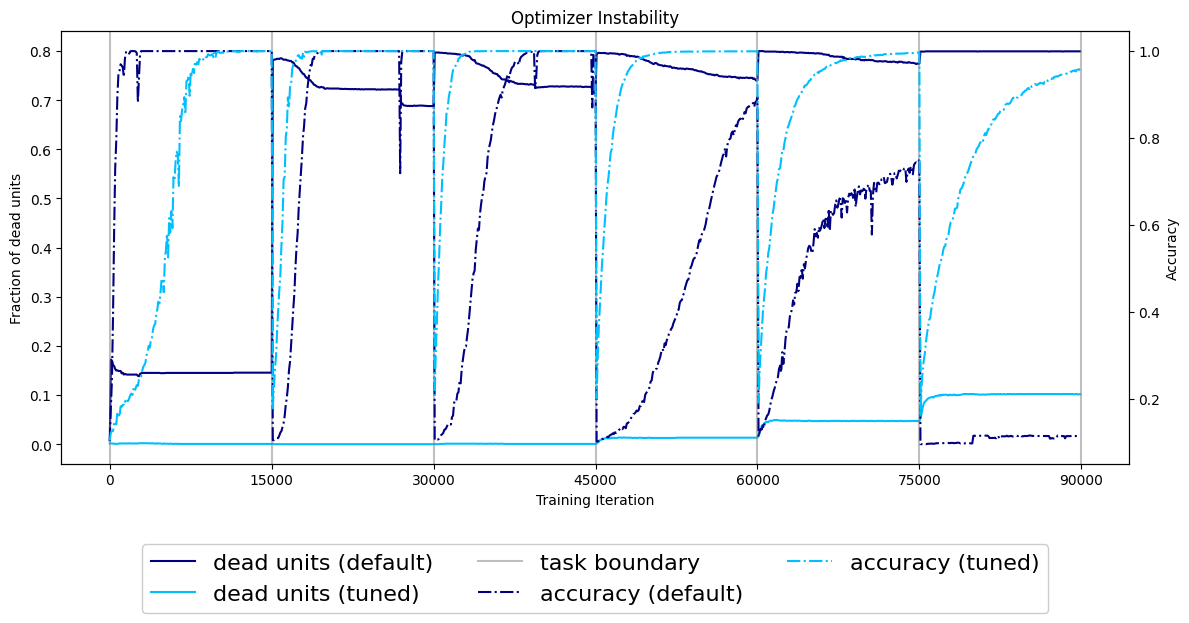
\includegraphics[width=0.9\textwidth]{assets/figure1.png}
% \fbox{\rule{0pt}{2.6in}\rule{0.85\linewidth}{0pt}}
\caption{Abrupt label changes destabilize Adam and lead to a large fraction of inactive ReLU units.}
\label{fig:result_optimizer_instability}
\end{figure}

\subsection{Hessian Spectrum and Gradient Covariance}

\begin{figure}[htbp]
\centering
% Replace with reproduced Figure 2
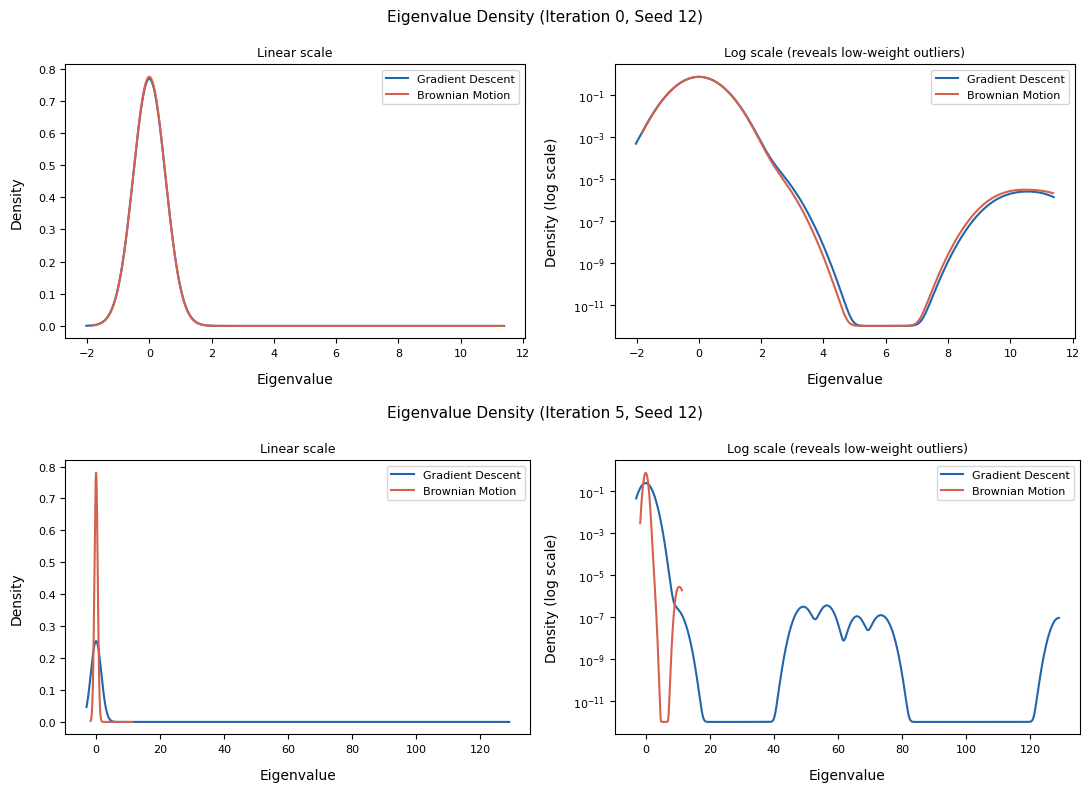
\includegraphics[width=0.85\textwidth]{assets/figure2_hessian.png}
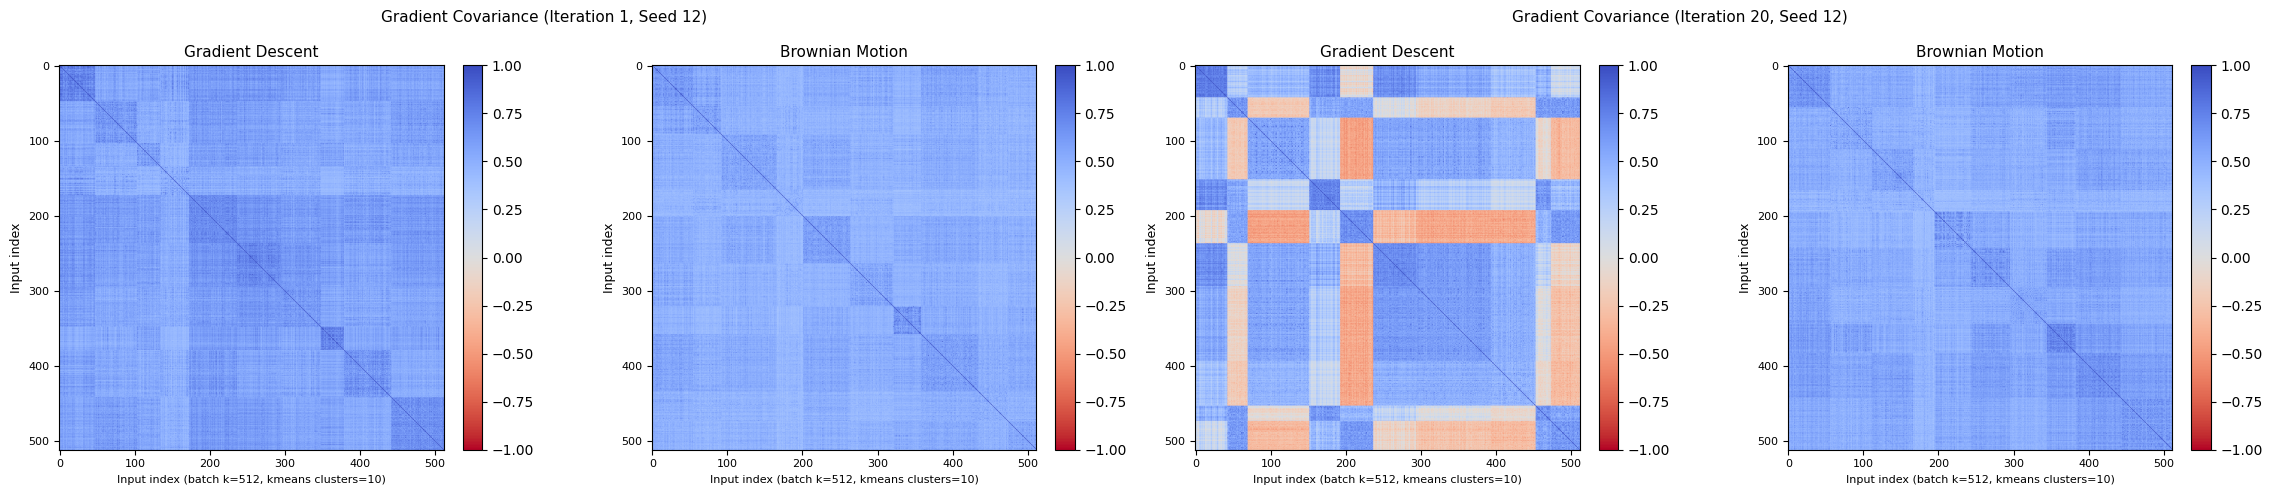
\includegraphics[width=0.85\textwidth]{assets/figure2_grad_cov.png}
% \fbox{\rule{0pt}{3.0in}\rule{0.85\linewidth}{0pt}}
\caption{Hessian spectra and gradient covariance matrices, in the beginning and after 20 epochs of training.}
\label{fig:result_hessian_gradient_covariance}
\end{figure}

The goal is to compare how the loss landscape evolves under gradient-based optimization versus random perturbations of the parameters. We use hessian curvature and gradient covariance to analyze the loss landscape. In both cases, the magnitude of the parameter change is controlled, but the direction of the update differs.

The Hessian spectrum is used to analyze the curvature of the probe loss landscape. Larger spectral outliers indicate sharper directions in parameter space and therefore potentially worse optimization conditioning. The reproduced Hessian analysis shows that gradient-based training tends to produce larger Hessian outliers than random Brownian perturbations. This suggests that training does not merely move the network away from initialization, but moves it in directions that make the local loss landscape harder to optimize.

Gradient covariance matrices are computed to analyze interference between samples.
Since the entries of the gradient covariance matrix are cosine similarities between normalized gradient vectors, their values must lie in the interval $[-1,1]$. Therefore, in the reproduced plots we use the corrected color range $[-1,1]$ rather than the wider range shown in the original visualization $[-5, 5]$.
In the gradient covariance heatmaps, positive values indicate aligned gradients, while negative values indicate gradient interference. We observe that after training for 20 epochs, the gradient covariance matrix shows more negative interference between samples compared to the initial state, meaning that the network cannot change its representation independently on many samples and directions. This suggests that gradient-based optimization can create a less favorable structure for adapting to new objectives, which may contribute to plasticity loss.

For clarity, we note that the Hessian and gradient covariance are computed using the probe loss, which is a separate loss function used to evaluate the network's ability to adapt to new objectives. This allows us to isolate the effects of training on the loss landscape from the specific task being learned.



\subsection{Falsification of Simple Explanations}

This experiment investigates whether previously proposed quantities such as weight norm and number of inactive units can provide a causal explanation of plasticity loss.

The key idea is that a true causal mechanism should show a consistent relationship with plasticity across different environments. However, the reproduced results show that these quantities do not behave consistently. In some settings, the correlation with plasticity loss is positive, while in others it is negative or weak. Therefore, these quantities may be correlated with plasticity loss in particular cases, but they do not provide a general causal explanation.

\begin{figure}[htbp]
\centering
% Replace with reproduced Figure 3

\includegraphics[width=0.85\textwidth]{assets/figure3_falsification.png}
% \fbox{\rule{0pt}{3.0in}\rule{0.85\linewidth}{0pt}}
\caption{Previously proposed explanations do not show a consistent relationship with plasticity loss across various environments.}
\label{fig:result_falsification}
\end{figure}

\subsection{Learning Curve Evolution on Probe Tasks}

The purpose of this experiment is to understand whether plasticity loss corresponds to poor local minima or to slower optimization progress on new objectives.

The reproduced learning curves show that networks from later training checkpoints reduce the probe loss more slowly than networks near initialization. This suggests that plasticity loss is expressed primarily as slower adaptation, rather than simply convergence to a worse final plateau.

\begin{figure}[htbp]
\centering
% Replace with reproduced Figure 4
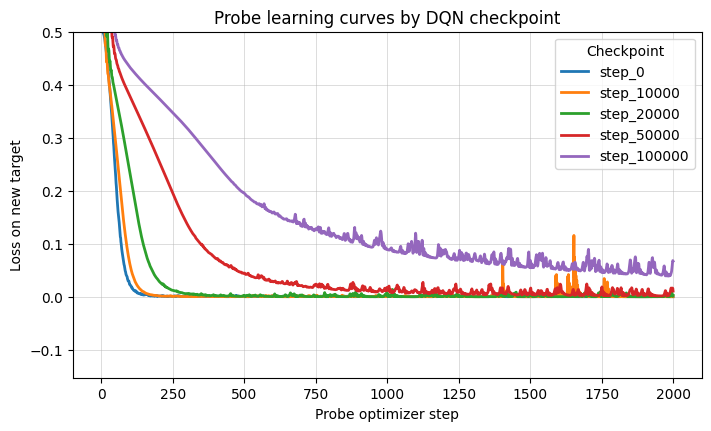
\includegraphics[width=0.85\textwidth]{assets/figure4_full_training.png}
% \fbox{\rule{0pt}{2.6in}\rule{0.85\linewidth}{0pt}}
\caption{Later checkpoints show slower optimization on probe tasks, indicating reduced plasticity.}
\label{fig:result_probe_learning_curves}
\end{figure}

\subsection{Effect of Network Width on Plasticity Loss}

This experiment studies whether increasing network width is sufficient to prevent plasticity loss.

The reproduced results indicate that wider networks generally suffer less plasticity loss than smaller networks. However, increasing width alone does not fully eliminate the problem. This suggests that plasticity loss is not merely a consequence of insufficient model capacity, but is also related to optimization dynamics and the geometry of the loss landscape.

\begin{figure}[htbp]
\centering
% Replace with reproduced Figure 5

\includegraphics[width=0.85\textwidth]{assets/figure5_width_sweep.png}
% \fbox{\rule{0pt}{2.6in}\rule{0.85\linewidth}{0pt}}
\caption{Increasing width reduces plasticity loss but does not fully remove it.}
\label{fig:result_width}
\end{figure}

\subsection{Effect of Plasticity-Preserving Interventions}

This experiment compares several interventions designed to reduce plasticity loss, including layer normalization, reset-based methods, shrink-and-perturb, weight decay, spectral normalization, and categorical output representations.

The reproduced results support the conclusion that interventions which improve the smoothness and conditioning of the loss landscape are the most effective. In particular, layer normalization and categorical output representations show strong improvements compared to methods that only perturb or regularize the parameters. This supports the broader hypothesis that plasticity loss is closely related to loss landscape geometry.

\begin{figure}[htbp]
\centering
% Replace with reproduced Figure 6

\includegraphics[width=0.85\textwidth]{assets/figure6_intervention_matrix.png}
% \fbox{\rule{0pt}{3.0in}\rule{0.85\linewidth}{0pt}}
\caption{Interventions that smooth or stabilize the loss landscape are most effective at preserving plasticity.}
\label{fig:result_interventions}
\end{figure}
